\documentclass[9pt,aspectratio=169,xcolor=table]{beamer}

%~~~~~~~~~~~~~~~~~~~~~~~~~~~~~~~~~~~~~~~~~~~~~~~~~~~~~~~~~~~~~~~~~~~~~~~~~~~~~~
% Use roboto Font (recommended)
\usepackage[sfdefault]{roboto}
\usepackage[utf8]{inputenc}
\usepackage[T1]{fontenc}
%~~~~~~~~~~~~~~~~~~~~~~~~~~~~~~~~~~~~~~~~~~~~~~~~~~~~~~~~~~~~~~~~~~~~~~~~~~~~~~

%~~~~~~~~~~~~~~~~~~~~~~~~~~~~~~~~~~~~~~~~~~~~~~~~~~~~~~~~~~~~~~~~~~~~~~~~~~~~~~
% Define where theme files are located. ('/styles')
\usepackage{styles/fluxmacros}
\usefolder{styles}
% Use Flux theme v0.1 beta
% Available style: asphalt, blue, red, green, gray
\usetheme[style=hunter]{flux}
%~~~~~~~~~~~~~~~~~~~~~~~~~~~~~~~~~~~~~~~~~~~~~~~~~~~~~~~~~~~~~~~~~~~~~~~~~~~~~~

%~~~~~~~~~~~~~~~~~~~~~~~~~~~~~~~~~~~~~~~~~~~~~~~~~~~~~~~~~~~~~~~~~~~~~~~~~~~~~~
% Extra packages
\usepackage{booktabs}
\usepackage{colortbl}
\usepackage{ragged2e}
\usepackage{amssymb}
\usepackage{multirow}
\usepackage{tikz}
\usetikzlibrary{arrows.meta, positioning, fit, backgrounds, calc, decorations.pathreplacing}
\setbeamertemplate{itemize items}[square]
\usepackage[scaled=.8]{beramono}
\usepackage{listings}
\usepackage{styles/lstlangarm}
\usepackage{array}
\definecolor{bgcolor}{HTML}{F2E9E9}
% lstlangarm.sty references \color{mauve} for string literals but never defines
% it -- only fires when a listing contains a string. Define it here.
\definecolor{mauve}{rgb}{0.58,0,0.82}
% lstlangarm's C style sets commentstyle=green!20, which is unreadable on the
% pink listing background. Darken it globally.
\lstset{commentstyle=\color{green!45!black}}
% ragged-right fixed-width column -- must be defined in the preamble, never
% inside a frame (\newcolumntype's #1 breaks beamer's frame scanner)
\newcolumntype{R}[1]{>{\RaggedRight\arraybackslash}p{#1}}
%~~~~~~~~~~~~~~~~~~~~~~~~~~~~~~~~~~~~~~~~~~~~~~~~~~~~~~~~~~~~~~~~~~~~~~~~~~~~~~
% Table striping: odd rows white, even rows very light gray.
% Needs \documentclass[...,xcolor=table]{beamer} (beamer loads xcolor itself,
% so the option must go on the class, not \usepackage).
\definecolor{stripe}{gray}{0.94}
% \striped makes body rows alternate white, gray, white, ... starting white.
% \rowcolors counts from the first coloured body row; the header is not counted.
\newcommand{\striped}{\rowcolors{1}{white}{stripe}}
%~~~~~~~~~~~~~~~~~~~~~~~~~~~~~~~~~~~~~~~~~~~~~~~~~~~~~~~~~~~~~~~~~~~~~~~~~~~~~~

%~~~~~~~~~~~~~~~~~~~~~~~~~~~~~~~~~~~~~~~~~~~~~~~~~~~~~~~~~~~~~~~~~~~~~~~~~~~~~~
% TikZ block styles -- matches ch1/ch2
% Colour variables are named identically in the book's stm32primer.tex, so any
% tikzpicture using only the \tikzset{...} styles below can be copied verbatim
% between slides and book. Only the \definecolor/\colorlet VALUES differ: the
% book is printed, so it keeps every stroke pure black with muted fills. These
% slides are projected, so both fill AND stroke are bright and saturated to
% grab attention -- see stm32primer.tex for the print palette.
\definecolor{blkfill}{HTML}{DDEEDD}
\definecolor{blkline}{HTML}{355E3B}
\definecolor{accentfill}{HTML}{FFE0B2}
\definecolor{accentline}{HTML}{E65100}
\definecolor{memfill}{HTML}{DFF5DA}
\definecolor{memline}{HTML}{2E7D32}
\definecolor{cellfill}{HTML}{FFFFFF}
\definecolor{cellline}{HTML}{424242}
\definecolor{bitmaskfill}{HTML}{DCEBFF}
\definecolor{bitmaskline}{HTML}{1565C0}
\definecolor{bithitfill}{HTML}{FFE0B2}
\definecolor{bithitline}{HTML}{E65100}
\tikzset{
  blk/.style   = {rectangle, rounded corners=2pt, draw=blkline, fill=blkfill,
                  thick, align=center, font=\small, minimum height=9mm, inner sep=3pt},
  cpublk/.style= {rectangle, rounded corners=2pt, draw=accentline, fill=accentfill,
                  thick, align=center, font=\small\bfseries, minimum height=9mm, inner sep=3pt},
  memblk/.style= {rectangle, rounded corners=2pt, draw=memline, fill=memfill,
                  thick, align=center, font=\small, minimum height=9mm, inner sep=3pt},
  cell/.style  = {rectangle, draw=cellline, fill=cellfill, align=center,
                  font=\small\ttfamily, minimum height=7mm, inner sep=2pt},
  bitcell/.style={rectangle, draw=cellline, fill=cellfill, thick,
                  minimum width=5.4mm, minimum height=5.4mm, inner sep=0pt,
                  font=\scriptsize\ttfamily, anchor=center},
  bitmask/.style={bitcell, fill=bitmaskfill, draw=bitmaskline},
  bithit/.style ={bitcell, fill=bithitfill, draw=bithitline, font=\scriptsize\ttfamily\bfseries},
  rowlab/.style ={font=\scriptsize, text=Gray, anchor=east},
  oplab/.style  ={font=\scriptsize\itshape, text=Gray, anchor=west},
  lbl/.style   = {font=\scriptsize, text=Gray},
  flow/.style  = {-{Stealth[length=2mm]}, thick, draw=blkline},
  busline/.style={thick, draw=cellline},
}
% NOTE (theme quirks -- all fail SILENTLY, always page through the PDF):
%  - a second \\ inside a nested {...} group in a TikZ node breaks parsing
%  - {\small ...} wrapped around a nested itemize eats the frame title + list
%  - \usebeamercolor on a [plain] frame falls through to an unstyled default
%  - \newcolumntype inside a frame breaks beamer's frame scanner
%  - lstlisting needs \begin{frame}[fragile]
%  - a TikZ picture wider than its column silently overflows into neighbours
%~~~~~~~~~~~~~~~~~~~~~~~~~~~~~~~~~~~~~~~~~~~~~~~~~~~~~~~~~~~~~~~~~~~~~~~~~~~~~~

%%%%%%%%%%%%%%%%%%%%%%%%%%%%%%%%%%%
%% BEGIN CONDITIONAL COMPILATION %%
%%%%%%%%%%%%%%%%%%%%%%%%%%%%%%%%%%%
\newif\ifwebex
%\webextrue % uncomment to generate section separator
\ifwebex
\AtBeginSection[]{
  \begin{frame}
  \vfill
  \centering
  \begin{beamercolorbox}[sep=8pt,center,shadow=true,rounded=true]{title}
    \usebeamerfont{title}\insertsectionhead\par%
  \end{beamercolorbox}
  \vfill
  \end{frame}
}
\else
\AtBeginSection[]
{
{
    \setbeamercolor{background canvas}{bg=yellow!10}
    \begin{frame}[plain]
        \frametitle{Table of Contents}
        \tableofcontents[currentsection]
    \end{frame}
}
}
\fi
%%%%%%%%%%%%%%%%%%%%%%%%%%%%%%%%%%%
%% END CONDITIONAL COMPILATION   %%
%%%%%%%%%%%%%%%%%%%%%%%%%%%%%%%%%%%

%~~~~~~~~~~~~~~~~~~~~~~~~~~~~~~~~~~~~~~~~~~~~~~~~~~~~~~~~~~~~~~~~~~~~~~~~~~~~~~
% Information
\title{Karnaugh Maps}
\subtitle{\emph{Contemporary Digital Electronic Systems} --- Chapter 6}
\author{Mun\'{i}m Zabidi}
\institute{\color{primary}Faculty of Electrical Engineering, Universiti Teknologi Malaysia}
\date{\today}
\titlegraphic{assets/logoutmwhite.png}
\graphicspath{{.}{assets/}}
%~~~~~~~~~~~~~~~~~~~~~~~~~~~~~~~~~~~~~~~~~~~~~~~~~~~~~~~~~~~~~~~~~~~~~~~~~~~~~~

\newcommand{\rulefig}[3]{\par\vspace{1mm}{\small\textbf{#1}\ #2}\par\vspace{.5mm}\centerline{\includegraphics[width=.62\textwidth]{#3}}}


% 4-variable K-map: \kmapfour{16 entries, row-major, rows AB=00,01,11,10; columns CD=00,01,11,10}
\newcommand{\kmapfour}[1]{%
  \begin{tikzpicture}[x=.75cm,y=.75cm,font=\sffamily\small]
    \foreach \c [count=\i from 0] in {00,01,11,10} \node at (\i+.5,.4) {\scriptsize\c};
    \foreach \r [count=\i from 0] in {00,01,11,10} \node at (-.5,-\i-.5) {\scriptsize\r};
    \node at (-.5,.4) {\scriptsize $AB\backslash CD$};
    \draw (0,0) grid (4,-4);
    \foreach \v [count=\k from 0] in {#1} {%
      \pgfmathtruncatemacro{\rr}{int(\k/4)}\pgfmathtruncatemacro{\cc}{mod(\k,4)}%
      \node at (\cc+.5,-\rr-.5) {\v};}
  \end{tikzpicture}}

\begin{document}

\titlepage

%===============================================================================
\section{Why This Chapter}
%===============================================================================

\begin{frame}{Why This Chapter Matters}
  \begin{columns}[c]
  \begin{column}{.47\textwidth}
    Boolean algebra simplifies by rewriting rules. It is error-prone and does not show whether the result is the \alert{smallest}. A Karnaugh map is a graphical procedure that finds a minimum SOP (or POS) directly from the truth table, for functions of up to four variables.
  \end{column}
  \begin{column}{.51\textwidth}
    \begin{block}{After this chapter, you can:}
    {\small
    \begin{enumerate}\itemsep2pt
      \item Lay out a 2-, 3- and 4-variable K-map in Gray-code order.
      \item Transfer a truth table into a K-map and back.
      \item Identify prime and essential prime implicants.
      \item Extract a minimum-cost SOP (or POS) expression.
      \item Use don't-cares to reduce the expression further.
    \end{enumerate}}
    \end{block}
  \end{column}
  \end{columns}
\end{frame}

\begin{frame}{An Opening Question}
  \leavevmode\vspace{4mm}
  \begin{center}
  \fbox{\parbox{.78\textwidth}{\centering\vspace{2mm}
  \large Why is the K-map laid out in \alert{Gray-code} order, not normal binary order?
  \vspace{2mm}}}
  \end{center}
  \vspace{4mm}
  What property of adjacent cells does that layout preserve? Keep this in mind as we build the maps.
\end{frame}

%===============================================================================
\section{Overview}
%===============================================================================

\begin{frame}{What Is a Karnaugh Map?}
  \begin{itemize}\itemsep3pt
    \item A \alert{K-map} (or Veitch diagram) is a truth table drawn as a 2-D grid. Each cell is one truth-table row.
    \item An $n$-variable map has $2^n$ cells.
    \item Best for small problems (up to four variables); impractical beyond that.
    \item Simpler expressions mean a simpler circuit, with more reliability and speed and lower cost.
    \item Two adjacent 1s always group: they differ in one variable $x$, and $x\cdot t + \overline{x}\cdot t = t$ by the unifying theorem, so $x$ drops out.
  \end{itemize}
  \centering
  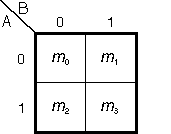
\includegraphics[height=.22\textheight]{kmap2vtype1}\hspace{8mm}
  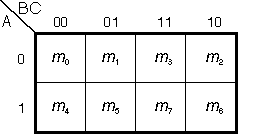
\includegraphics[height=.22\textheight]{kmap3vtype1}\\[1mm]
  {\small 2-variable map ($m_0$ to $m_3$) \hspace{.1\textwidth} 3-variable map ($m_0$ to $m_7$)}
\end{frame}

\begin{frame}{Gray-Code Order Keeps Neighbours Adjacent}
  \begin{columns}[c]
  \begin{column}{.55\textwidth}
    \begin{itemize}\small\itemsep3pt
      \item Rows and columns follow Gray-code order, so the minterm indices of adjacent cells differ in \alert{exactly one bit}.
      \item Adjacent cells differ in one variable. That variable can be eliminated when they are grouped.
      \item This answers the opening question.
      \item A 2-variable function has only $2^{2^2} = 16$ possible maps, so those maps have limited use.
    \end{itemize}
  \end{column}
  \begin{column}{.43\textwidth}
    \centering
    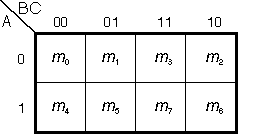
\includegraphics[width=.9\textwidth]{kmap3vtype1}
  \end{column}
  \end{columns}
\end{frame}

\begin{frame}{Filling in a K-Map}
  \begin{columns}[c]
  \begin{column}{.5\textwidth}
    \begin{block}{$F = AB + AC$}
      \small
      Convert to canonical SOP first:\\
      $= AB(C+\overline{C}) + AC(B+\overline{B})$\\
      $= A\overline{B}C + AB\overline{C} + ABC$\\
      $= \sum m(5,6,7)$
    \end{block}
    \centering
    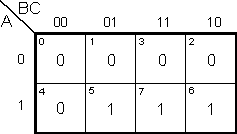
\includegraphics[width=.55\textwidth]{kmap3v_ex2}
  \end{column}
  \begin{column}{.48\textwidth}
    \begin{block}{Prime numbers 0 to 7}
      \small Primes: 2, 3, 5, 7. So $F = 1$ at $m_2, m_3, m_5, m_7$.
    \end{block}
    \centering
    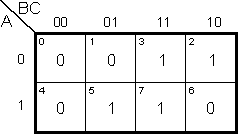
\includegraphics[width=.55\textwidth]{kmap3v_ex1a}
  \end{column}
  \end{columns}
\end{frame}

%===============================================================================
\section{Minimization with K-Maps}
%===============================================================================

\begin{frame}{Grouping Adjacent Cells}
  \begin{columns}[c]
  \begin{column}{.55\textwidth}
    \begin{itemize}\small\itemsep3pt
      \item Two adjacent minterms differ in one variable, so by the unifying theorem $A + \overline{A} = 1$ that variable disappears:
    \end{itemize}
    \[ A\overline{B}C + ABC = AC(\overline{B}+B) = AC \]
    \begin{itemize}\small\itemsep3pt
      \item A loop of $2^n$ cells eliminates $n$ variables. Larger loops give simpler terms.
      \item Cells on opposite edges are also adjacent: the map wraps around.
    \end{itemize}
  \end{column}
  \begin{column}{.43\textwidth}
    \centering
    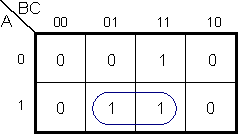
\includegraphics[width=.8\textwidth]{kmap3v_ex3}
  \end{column}
  \end{columns}
\end{frame}

\begin{frame}{Example Loops (3 Variables)}
  \centering
  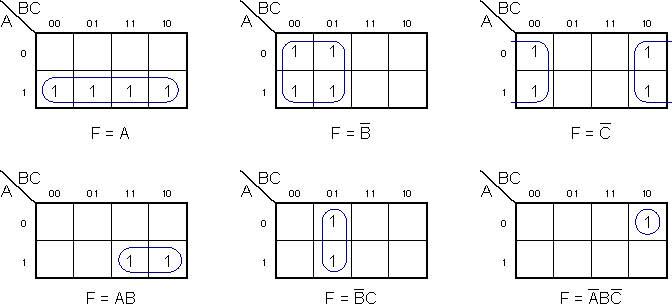
\includegraphics[width=.8\textwidth]{kmap3v_exloops}
  \begin{itemize}\small
    \item Only cells containing 1 are looped.
    \item The grouping for $F = \overline{C}$ shows the wraparound property.
  \end{itemize}
\end{frame}

\begin{frame}{K-Map Simplification Procedure}
  \begin{enumerate}\itemsep4pt
    \item Place all minterms on the map and mark the cells containing 1.
    \item Form rectangular loops of $2^n$ cells (1, 2, 4, 8, \dots).
    \item Always choose the \alert{largest} possible loops.
    \item A cell may belong to more than one loop if that gives a simpler result.
    \item Continue until every 1 is in at least one loop.
    \item Write one product term per loop and OR the terms together.
  \end{enumerate}
\end{frame}

\begin{frame}{Example: $F = \sum m(0,1,2,4,6)$}
  \begin{columns}[c]
  \begin{column}{.5\textwidth}
    \centering
    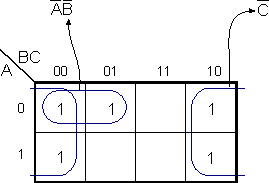
\includegraphics[width=.55\textwidth]{kmap3v_ex4}
  \end{column}
  \begin{column}{.48\textwidth}
    \begin{itemize}\small\itemsep3pt
      \item Loop of four: $m_0, m_2, m_4, m_6$. $A$ and $B$ change, $C = 0$: term $\overline{C}$.
      \item Pair: $m_0, m_1$. Only $C$ changes: term $\overline{A}\,\overline{B}$.
    \end{itemize}
    \begin{block}{Result}
      $F = \overline{A}\,\overline{B} + \overline{C}$
    \end{block}
  \end{column}
  \end{columns}
\end{frame}

%===============================================================================
\section{Eight Golden Rules}
%===============================================================================

\begin{frame}{Rules 1 and 2}
  \rulefig{Rule 1: No zeros allowed.}{A group may not contain a cell with 0: it would assert an output the truth table says is 0.}{kmap_error1}
  \rulefig{Rule 2: No diagonals.}{Adjacent cells differ in one variable, so it cancels; diagonal cells differ in two, so nothing cancels.}{kmap_error2}
\end{frame}

\begin{frame}{Rule 3: Only Powers of 2}
  \rulefig{Rule 3.}{A group of $2^k$ cells drops exactly $k$ variables, so sizes must be 1, 2, 4, 8, \ldots}{kmap_error3}
  \rulefig{}{A group of 3 or 6 cells is not allowed.}{kmap_error4}
\end{frame}

\begin{frame}{Rules 4 and 5}
  \rulefig{Rule 4: Each group as large as possible.}{A smaller group is still correct but \emph{not minimal}.}{kmap_error5}
  \rulefig{Rule 5: Every 1 must be in at least one group.}{An uncovered 1 would give output 0 for that input.}{kmap_error6}
\end{frame}

\begin{frame}{Rules 6 and 7}
  \rulefig{Rule 6: Groups may overlap.}{Covering a cell twice is harmless ($A + A = A$) and often lets groups grow larger.}{kmap_error7}
  \rulefig{Rule 7: Groups may wrap around.}{Left edge with right edge; top with bottom.}{kmap_error8}
\end{frame}

\begin{frame}{Rule 8 and Prime Implicants}
  \begin{columns}[c]
  \begin{column}{.5\textwidth}
    \rulefig{Rule 8: Fewest groups.}{A small group inside a bigger one adds an unnecessary gate.}{kmap_error9}
  \end{column}
  \begin{column}{.48\textwidth}
    \begin{itemize}\small\itemsep3pt
      \item A \alert{prime implicant} is a group of 1s obeying Rules 1--3 and 7 that cannot be enlarged (Rule 4).
      \item An \alert{essential prime implicant} covers a 1 that no other prime implicant covers. It must appear in every minimum SOP.
    \end{itemize}
  \end{column}
  \end{columns}
\end{frame}

\begin{frame}{Using Prime Implicants}
  \begin{enumerate}\itemsep5pt
    \item Circle all prime implicants.
    \item Select every essential prime implicant. Leaving one out would leave a 1 uncovered (Rule 5).
    \item If any 1s remain uncovered, add the fewest other prime implicants that cover them (Rule 8).
  \end{enumerate}
\end{frame}

%===============================================================================
\section{Four-Variable Maps}
%===============================================================================

\begin{frame}{The Four-Variable Map}
  \begin{columns}[c]
  \begin{column}{.4\textwidth}
    \centering
    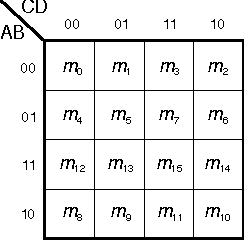
\includegraphics[width=.9\textwidth]{kmap4x4type1}
  \end{column}
  \begin{column}{.58\textwidth}
    \begin{itemize}\small\itemsep3pt
      \item $2^4 = 16$ cells, numbered $m_0$ to $m_{15}$.
      \item Rows and columns are in Gray-code order, so the map wraps horizontally and vertically.
      \item The four corners are adjacent to each other.
      \item Loops of 1, 2, 4, 8 or 16 cells eliminate 0 to 4 variables.
    \end{itemize}
  \end{column}
  \end{columns}
\end{frame}

\begin{frame}{Four-Variable Loops}
  \centering
  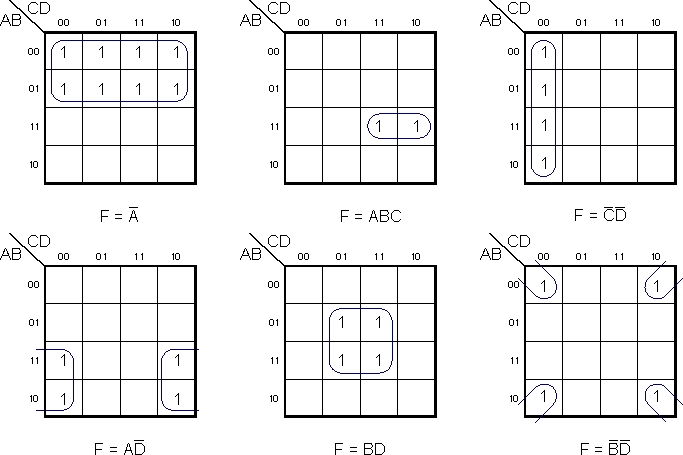
\includegraphics[height=.62\textheight]{kmap4v_exloops}
  \begin{itemize}\small
    \item A few of the possible coverings of a four-variable map.
  \end{itemize}
\end{frame}

\begin{frame}{Example: $F = \sum m(2,5,9,11,13,15)$}
  \begin{columns}[c]
  \begin{column}{.5\textwidth}
    \centering
    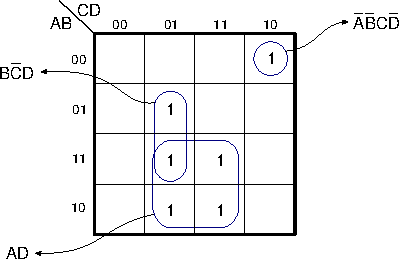
\includegraphics[width=\textwidth]{kmap234t}
  \end{column}
  \begin{column}{.48\textwidth}
    \begin{itemize}\small\itemsep3pt
      \item $m_9, m_{11}, m_{13}, m_{15}$: $A = 1,\ D = 1$, term $AD$.
      \item $m_5$ with $m_{13}$: term $B\overline{C}D$.
      \item $m_2$ has no neighbour: $\overline{A}\,\overline{B}C\overline{D}$.
    \end{itemize}
    \begin{block}{Result}
      $F = AD + B\overline{C}D + \overline{A}\,\overline{B}C\overline{D}$
    \end{block}
  \end{column}
  \end{columns}
\end{frame}

\begin{frame}{Example: Wraparound at the Corners}
  \begin{columns}[c]
  \begin{column}{.42\textwidth}
    \centering
    \kmapfour{1,0,0,1, 0,0,0,0, 0,0,0,0, 1,0,0,1}\\[1mm]
    {\small $F = \sum m(0,2,8,10)$}
  \end{column}
  \begin{column}{.56\textwidth}
    \begin{itemize}\small\itemsep3pt
      \item Rule 7: left and right columns are adjacent, as are top and bottom rows.
      \item The four corners touch and form \alert{one} group of four.
      \item $B = 0$ and $D = 0$ in all four cells; $A$ and $C$ take both values and cancel.
    \end{itemize}
    \begin{block}{Result}
      $F = \overline{B}\,\overline{D}$
    \end{block}
    \small Without wraparound: four isolated 1s and four four-literal terms.
  \end{column}
  \end{columns}
\end{frame}

%===============================================================================
\section{Don't Cares and POS}
%===============================================================================

\begin{frame}{Don't-Care Cells}
  \begin{itemize}\small\itemsep3pt
    \item Some inputs never occur, or their output does not matter: \alert{don't cares}, drawn as $\times$.
    \item A don't care may be treated as 1 if it enlarges a group; otherwise treat it as 0 and ignore it.
    \item Covering a don't care is optional.
  \end{itemize}
  \begin{block}{$F = \sum m(2,6,7) + \sum d(3,5)$}
    \small Set $m_3 = 1$ and $m_5 = 0$: the loop $m_2, m_3, m_6, m_7$ gives $F = B$.
  \end{block}
  \centering
  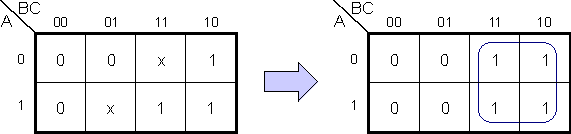
\includegraphics[height=.17\textheight]{kmap_dontcare}
\end{frame}

\begin{frame}{Example: Using Don't Cares}
  \begin{columns}[c]
  \begin{column}{.42\textwidth}
    \centering
    \kmapfour{0,1,1,0, 0,$\times$,1,0, 0,$\times$,1,0, 0,$\times$,1,0}\\[1mm]
    {\small $F = \sum m(1,3,7,11,15) + \sum d(5,9,13)$}
  \end{column}
  \begin{column}{.56\textwidth}
    \begin{itemize}\small\itemsep3pt
      \item 1s only: $F = CD + \overline{A}\,\overline{B}D$ (6 literals).
      \item Treat the don't cares as 1s: cells 1, 3, 5, 7, 9, 11, 13, 15 are exactly the eight cells with $D = 1$.
      \item One group of eight drops three variables.
    \end{itemize}
    \begin{block}{Result}
      $F = D$
    \end{block}
    \small A don't care that does not enlarge a group is left as 0.
  \end{column}
  \end{columns}
\end{frame}

\begin{frame}{K-Maps for Maxterms (POS)}
  \begin{columns}[c]
  \begin{column}{.52\textwidth}
    \centering
    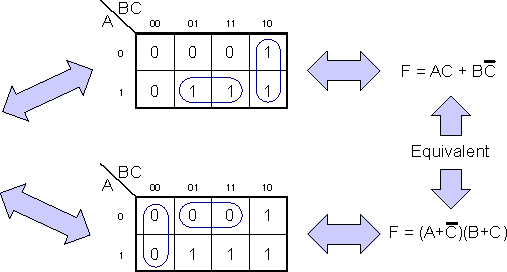
\includegraphics[width=\textwidth]{kmap_pos}
  \end{column}
  \begin{column}{.46\textwidth}
    \begin{itemize}\small\itemsep3pt
      \item Use the \alert{0} cells. Write a sum term per group, with complemented/uncomplemented roles swapped.
      \item SOP: $F = AC + B\overline{C}$.
      \item Zeros $M_1, M_3$: $(A+B+\overline{C})(A+\overline{B}+\overline{C}) = A+\overline{C}$.
      \item Zeros $M_0, M_4$: $(A+B+C)(\overline{A}+B+C) = B+C$.
    \end{itemize}
    \begin{block}{Result}
      $F = (A+\overline{C})(B+C)$
    \end{block}
  \end{column}
  \end{columns}
\end{frame}

\begin{frame}{Back to the Opening Question}
  \begin{block}{Why Gray-code order?}
    \small In Gray-code order, cells that are neighbours on the map differ in exactly one variable. That is what lets a group of adjacent 1s drop a variable. In plain binary order, neighbours such as 01 and 10 differ in two variables, so the unifying theorem would not apply.
  \end{block}
\end{frame}

%===============================================================================
\section{Summary}
%===============================================================================

\begin{frame}{Summary}
  \begin{itemize}\itemsep3pt\small
    \item Adjacent cells differ in one variable. Grouping $2^k$ adjacent 1s eliminates $k$ variables.
    \item Use the \alert{largest} groups and the \alert{fewest} groups.
    \item An \alert{essential prime implicant} covers a 1 no other prime implicant covers and must appear in every minimum SOP.
    \item Use \alert{don't-cares} when they allow larger groups; covering them is optional.
    \item For POS, group the 0s and write a sum term for each group.
  \end{itemize}
  \begin{block}{Looking ahead}
    Chapter 7 applies K-maps to complete combinational design problems.
  \end{block}
\end{frame}

\end{document}
